\documentclass[../main.tex]{subfiles}

\begin{document}

\subsection{Generación y validación de resúmenes modelo}

Se generaron un total de 50 resúmenes a partir de los historiales clínicos seleccionados.
Los expertos evaluaron la calidad de los resúmenes en términos de precisión, claridad y completitud de la información. Aunque eran distinguibles a simple vista con los resúmenes hechos a manos por los profesionales, estos contennían los contenidos y estructura adecuada.

Estos resultados respaldan el uso de los resúmenes modelo como referencia válida para la posterior evaluación automática del sistema de generación.

\subsection{Comparación de modelos SLM con resúmenes de referencia}

En esta sección se presentan los resultados obtenidos al evaluar los distintos modelos de lenguaje de menor tamaño en comparación con los resúmenes de referencia generados por GPT-4o-mini. El rendimiento de cada modelo se midió utilizando varias métricas automáticas de similitud, así como la complejidad temporal asociada con cada uno de los modelos.

\subsubsection{Métricas de similitud}

Se obtuvieron las métricas de similitud entre las 3000 respuestas generadas y las respuestas de referencia. Las métricas utilizadas incluyen BLEU, ROUGE y BERTScore.

Los resultados de las métricas de similitud por temperatura se resumen en la tabla \ref{tab:metricas_temperatura} donde no se observa a penas diferencia entre las dos temperaturas elegidas. 

\begin{table}[H]
    \centering
    \caption{Media de las métricas por temperatura}
    \label{tab:metricas_temperatura}
    \renewcommand{\arraystretch}{1.2}
    \begin{tabular}{c|ccccccc}
        \hline
        \textbf{Temperatura} & \textbf{BLEU} & \textbf{ROUGE1} & \textbf{ROUGE2} & \textbf{ROUGEL} & \textbf{BERT\_P} & \textbf{BERT\_R} & \textbf{BERT\_F1} \\
        \hline
        0.2 & 0.082000 & 0.253000 & 0.082000 & 0.136000 & 0.700000 & 0.692000 & 0.695000 \\
        0.8 & 0.082000 & 0.263000 & 0.083000 & 0.137000 & 0.698000 & 0.691000 & 0.694000 \\
        \hline
    \end{tabular}

\end{table}

En la Figura \ref{fig:metricas_por_modelo} se observan las métricas por modelo. Aunque en general obtienen resultados similares, el modelo que obtiene el mejor desempeño es \textbf{Phi-4}, seguido de \textbf{LLaMa3.2} y \textbf{Mistral}. 
Si bien actualmente no existe una gran cantidad de estudios sobre el uso de Phi-4 en el ámbito clínico, los resultados aquí obtenidos coinciden con estudios previos que reportan buen desempeño de Mistral \parencite{zhang2024mistral} y LLaMA \parencite{ji2024llama3deepseek} en tareas relacionadas con procesamiento de lenguaje biomédico.

\begin{figure}[H]
    \centering
    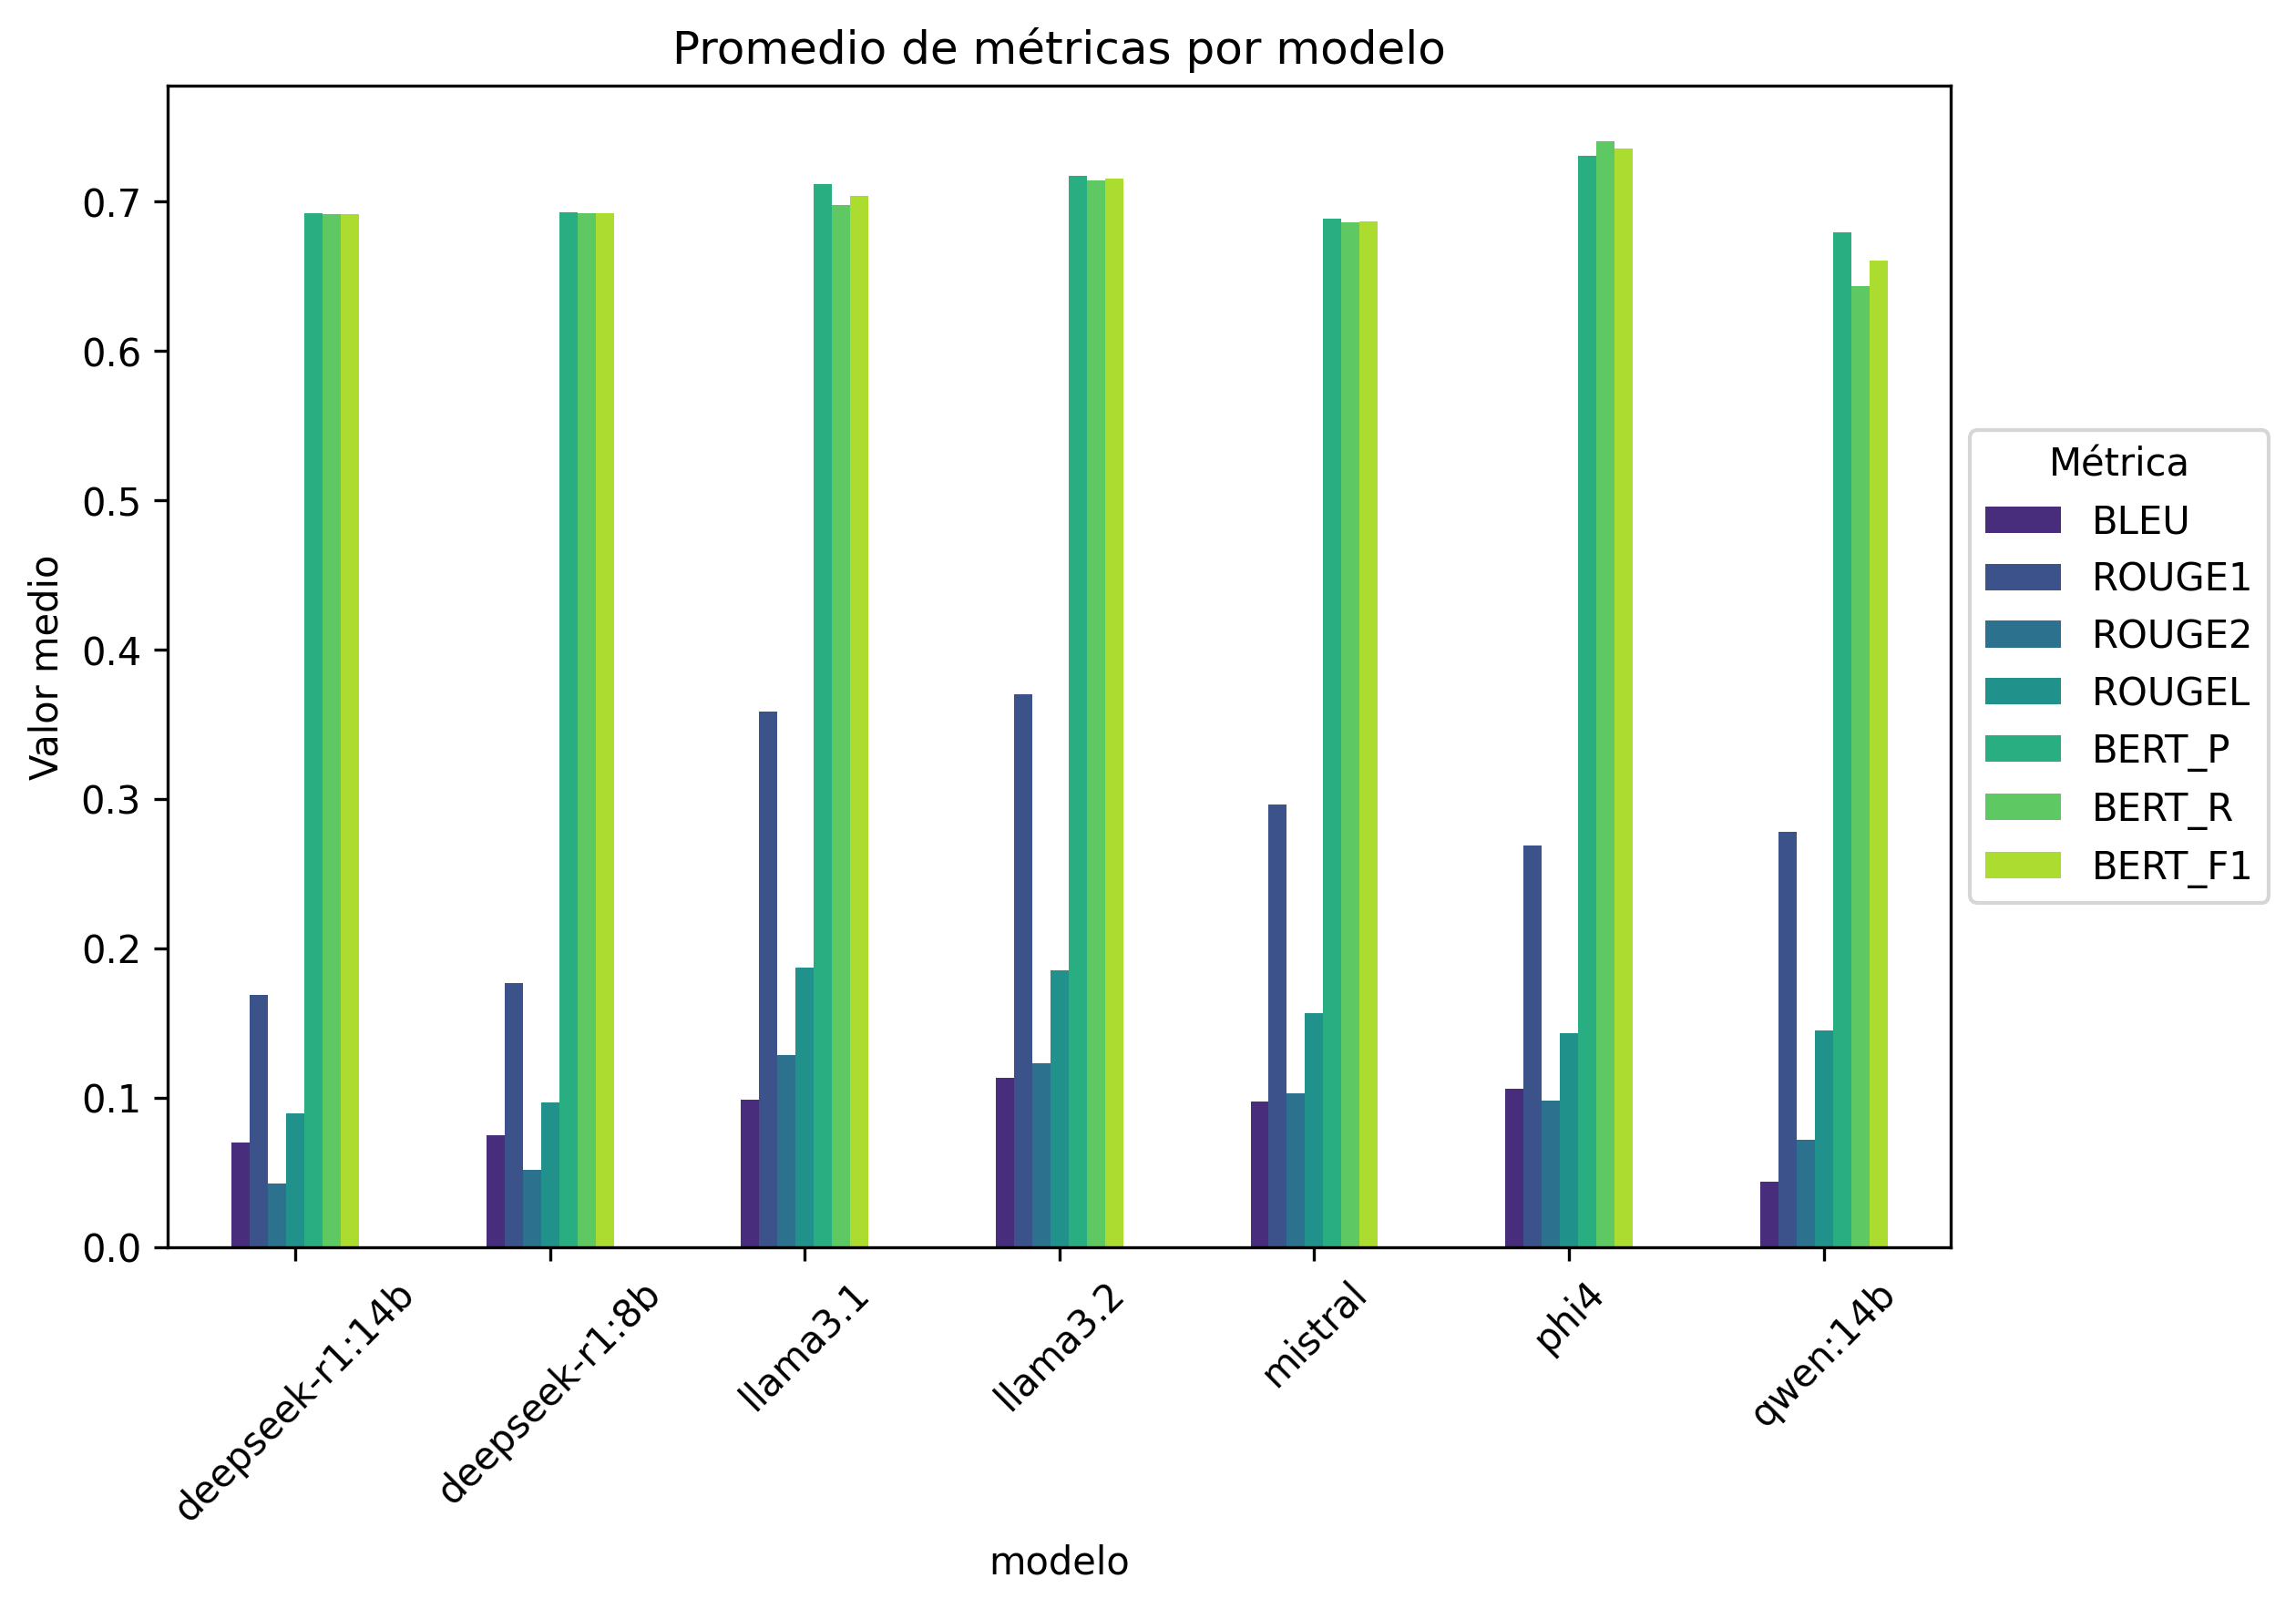
\includegraphics[width=0.8\textwidth]{images/metricas_por_modelo.png}
    \caption{Métricas por modelo. Comparación de los modelos evaluados según las métricas BLEU, ROUGE y BERTScore.}
    \label{fig:metricas_por_modelo}
\end{figure}

En la figura \ref{fig:metricas_por_contexto_modelos} se observan las métricas por contexto, siendo bastante parecidas. La técnica de prompting de generación por partes sobresale con unos resultados ligeramente mejores en todas las métricas y modelos. Esto se debe a que al segmentar el historial de entrada, la ventana de contexto de los modelos no se ven desbordadas tan facilmente.

\begin{figure}[H]
    \centering
    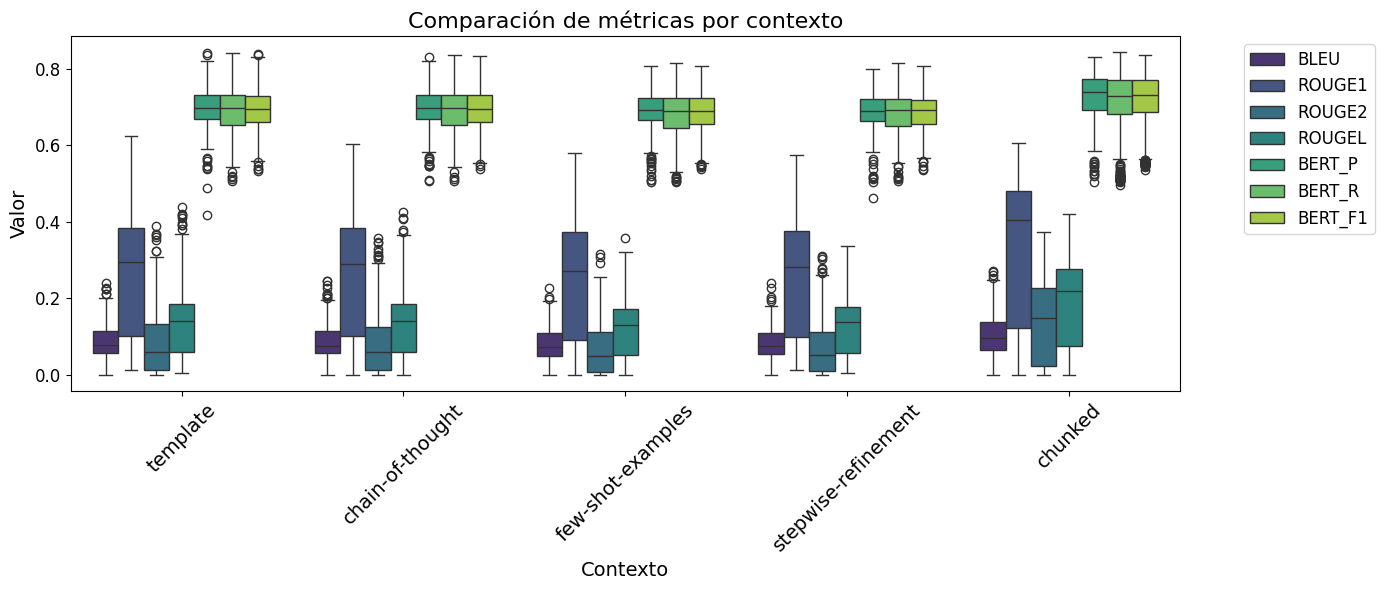
\includegraphics[width=0.8\textwidth]{images/metricas_por_contexto.png}
    \caption{Métricas por contexto. Comparación de las métricas de similitud según el contexto utilizado.}
    \label{fig:metricas_por_contexto}
\end{figure}

En las figuras \ref{fig:metricas_por_contexto_modelos} y  \ref{fig:metricas_por_contexto_deepseek} se observan las métricas por modelo y contexto. Destaca el modelo phi4 y mistral, la estrategia de prompt por partes es la que mejor funciona con estos modelos. Parece que los modelos con ventanas de contexto más grandes como los destilados de deepseek no se benefician tanto de la segmentación del historial.

\begin{figure}[H]
    \centering
    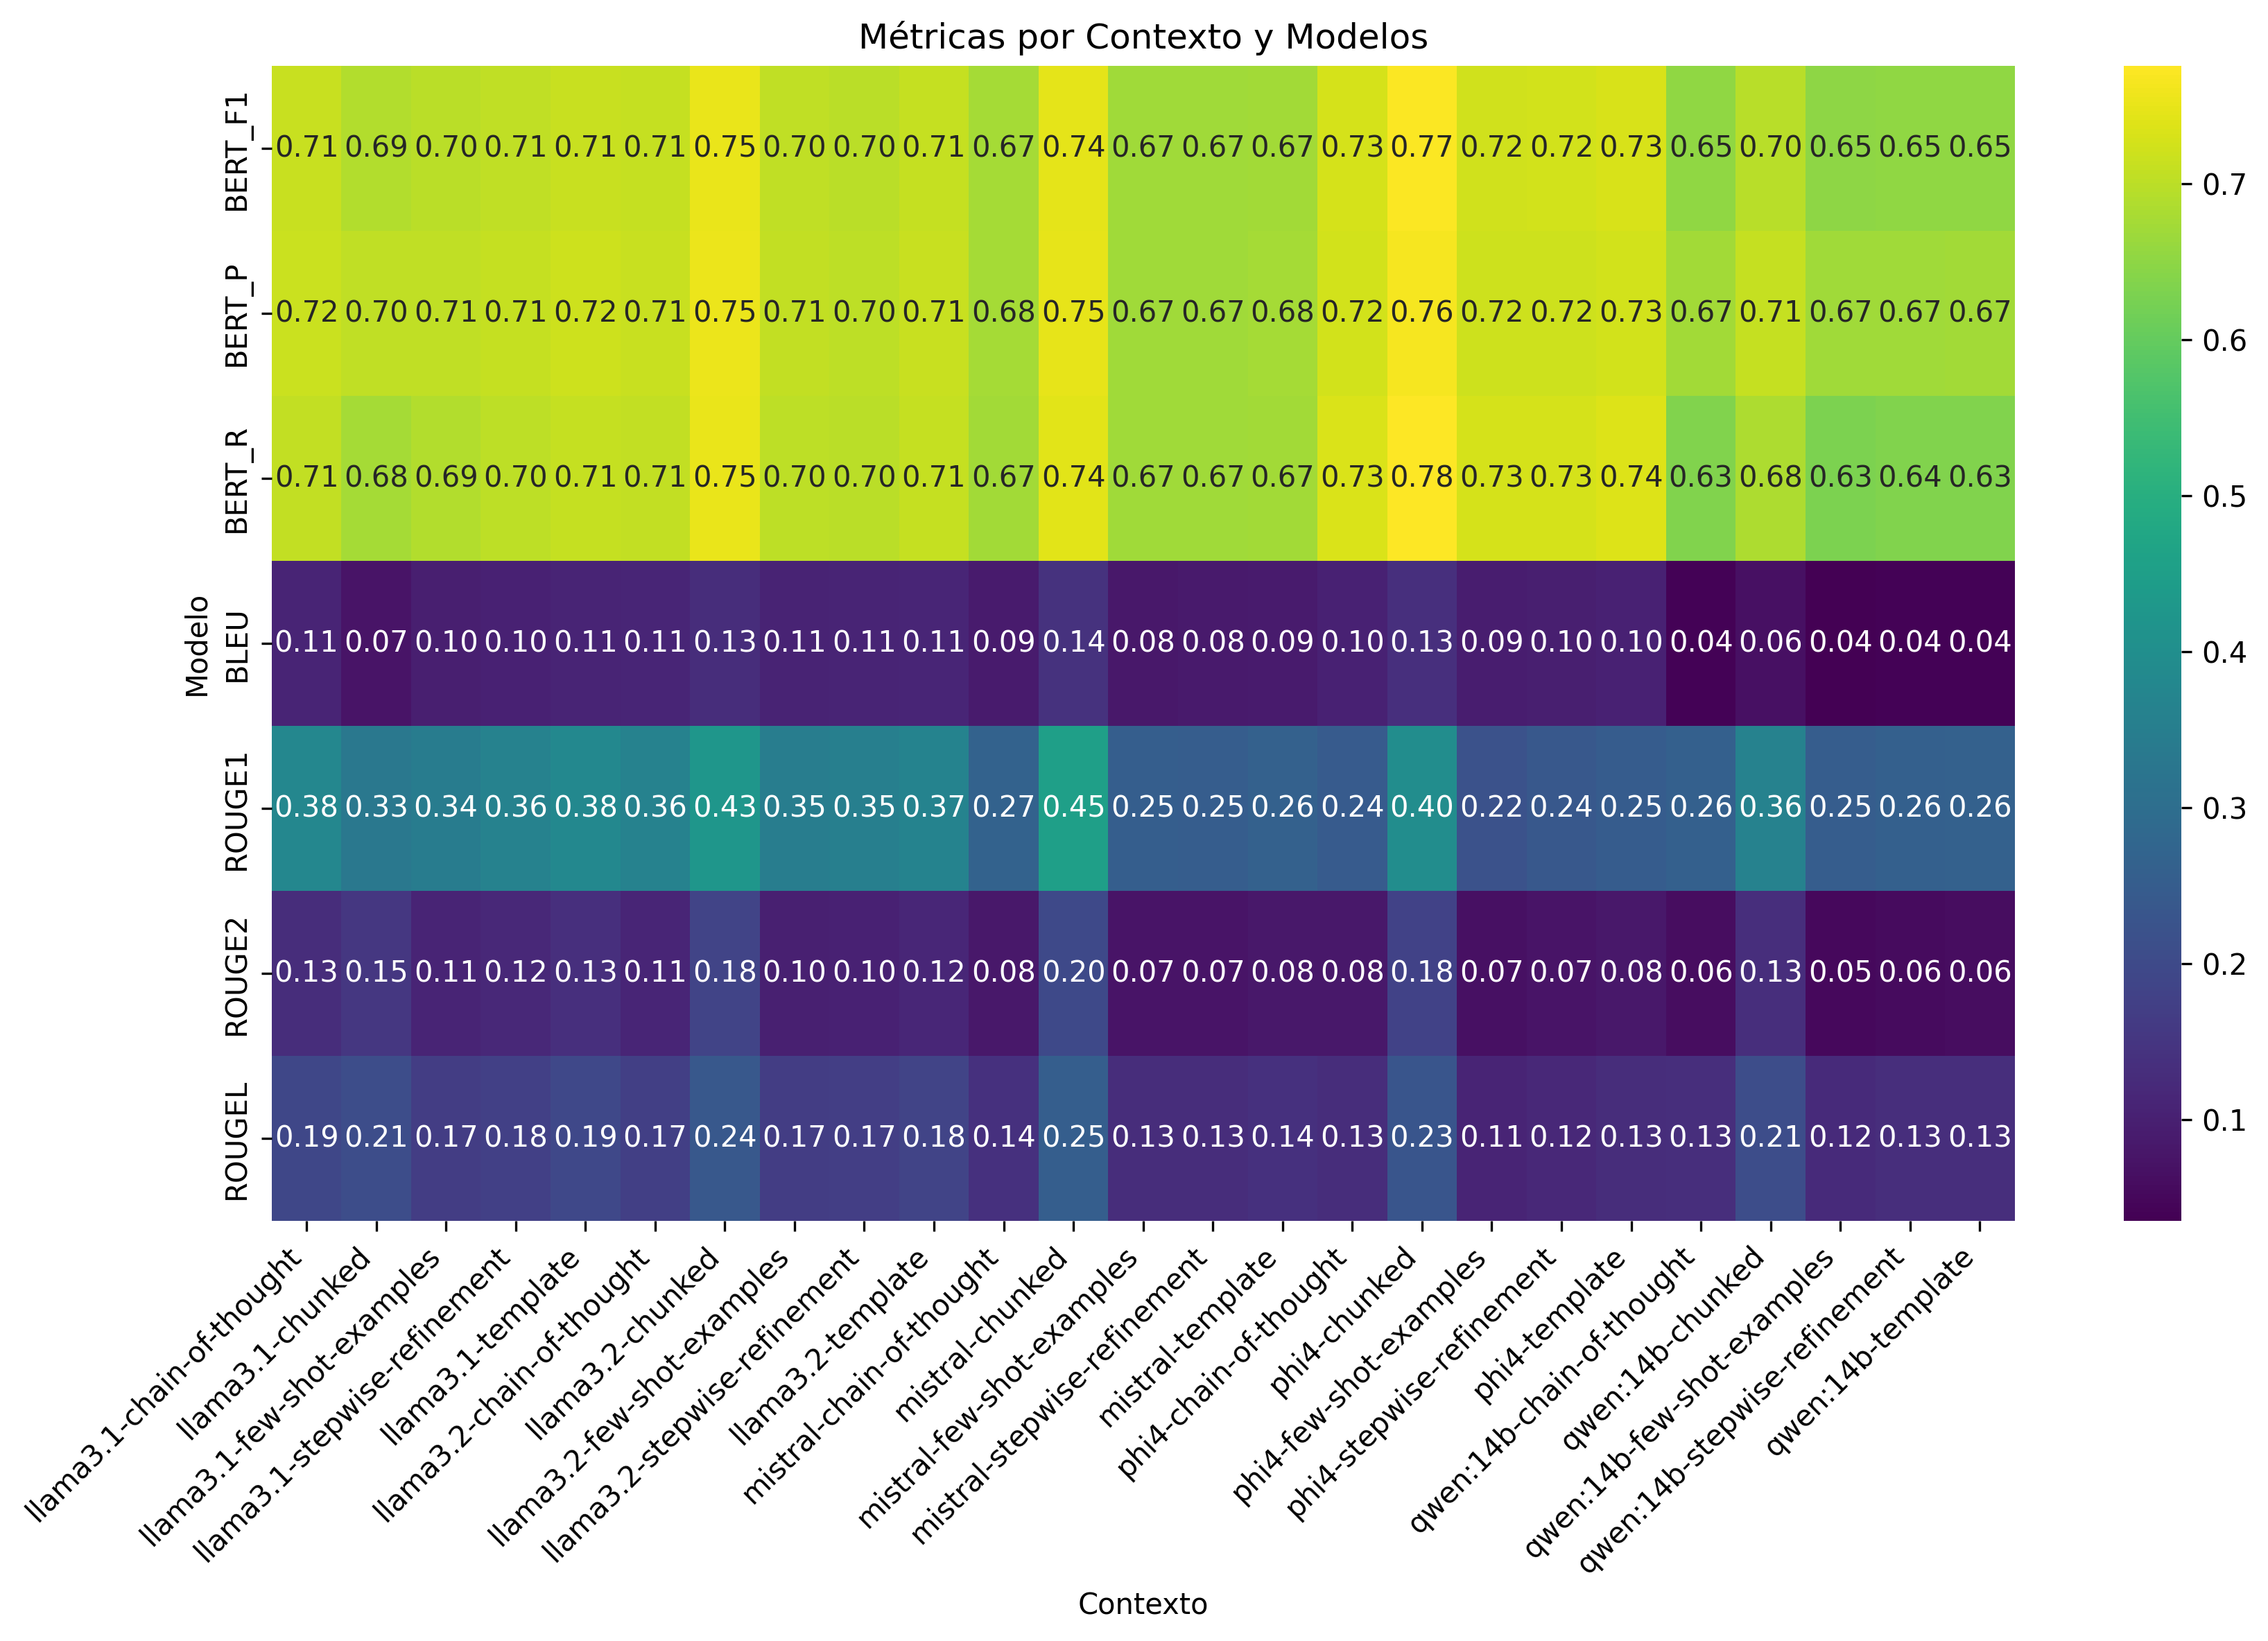
\includegraphics[width=0.8\textwidth]{images/metricas_por_contexto_modelos.png}
    \caption{Métricas por contexto y modelos. Comparación de las métricas de similitud para los distintos modelos bajo los mismos contextos.}
    \label{fig:metricas_por_contexto_modelos}
\end{figure}

\begin{figure}[H]
    \centering
    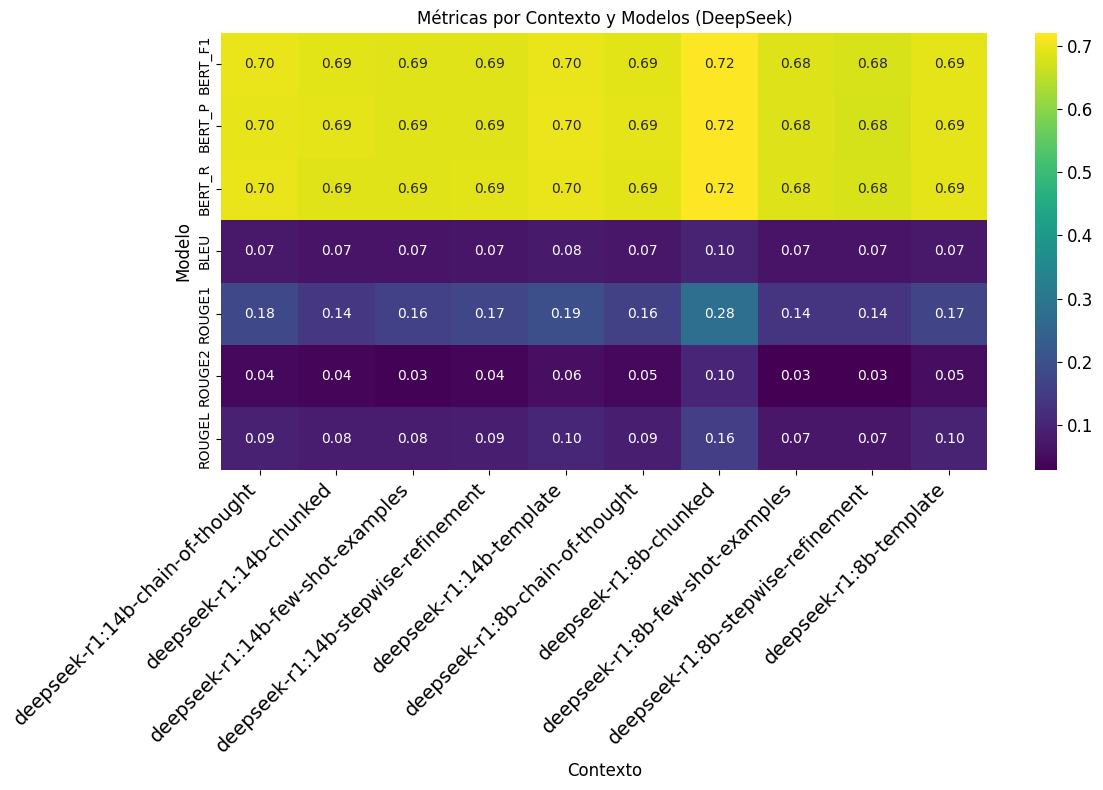
\includegraphics[width=0.8\textwidth]{images/metricas_por_contexto_deepseek.png}
    \caption{Métricas por contexto y Deepseek. Comparación de las métricas de similitud para el modelo Deepseek bajo diferentes contextos.}
    \label{fig:metricas_por_contexto_deepseek}
\end{figure}

\subsubsection{Tiempo de inferencia}

En cuanto a la complejidad temporal, se midió el tiempo de inferencia de cada uno de los modelos evaluados para determinar su eficiencia en la ejecución.

En la tabla \ref{tab:modelos_tiempo} se observa como hay una gran variación en el tiempo de inferencia, siendo los modelos destilados por deepseek varias veces mayores a los base. El mayor tiempo medio de inferencia es el destilado de qwen por deepseek siendo 386 segundos y el menor llama3.2 con 18 segundos.
Teniendo en cuenta que al hacer una inferencia por partes el tiempo necesario es el tiple, se decidió que phi4 seguía siendo el candidato ideal, ya que se prioriza la exactitud del modelo que el tiempo de respuesta.

\begin{table}[H]
    \centering
    \caption{Tiempo de ejecución por modelo}
    \label{tab:modelos_tiempo}
    \renewcommand{\arraystretch}{1.2}
    \begin{tabular}{ccc}
        \hline
        \textbf{Modelo} & \textbf{Media} & \textbf{Desviación} \\
        \hline
        deepseek-r1:8b & 157.26 & 85.74 \\
        deepseek-r1:14b & 386.24 & 182.28 \\
        llama3.1 & 48.2 & 37.64 \\
        llama3.2 & 18.2 & 3.23 \\
        qwen:14b & 42.61 & 2.65 \\
        mistral & 60.98 & 60.25 \\
        phi4 & 172.79 & 47 \\
        
        \hline
    \end{tabular}

\end{table}


\subsection{Implementación de modelo final}
\subsubsection{RAG}

En la Tabla \ref{tab:metricas_RAG} se presentan las métricas obtenidas por el modelo Phi-4 utilizando generación por partes junto con el sistema RAG multipregunta. El sistema alcanzó resultados sólidos en calidad de resumen, ligeramente mayores a los resultados sin RAG, con tiempos de ejecución de 523 segundos. Este valor incluye el tiempo requerido para realizar la búsqueda en la base de datos vectorial y ejecutar tres inferencias por segmento del historial clínico. Aunque el proceso implica un mayor coste computacional, la arquitectura permite que algunas fases, como la inferencia inicial de ideas clave, puedan ser ejecutadas en paralelo, lo cual abre la posibilidad de optimizar el rendimiento en futuras implementaciones.

Se ha confirmado que el sistema RAG es capaz de obtener información de contexto útil de la fuente de datos, no obstante, sería óptimo que en esta fuente de datos encontrásemos historias clínicas resumidas en lugar de ptreguntas y respuestas, de este modo el modelo podría encontrar contexto de cómo se suele resumir una parte del historial clínico con varios ejemplos.
\begin{table}[H]
	\centering
	\caption{Métricas obtenidas por RAG}
	\label{tab:metricas_RAG}
	\renewcommand{\arraystretch}{1.2}
	\begin{tabular}{c|cccccccc}
		\hline
		& \textbf{BLEU} & \textbf{ROUGE1} & \textbf{ROUGE2} & \textbf{ROUGEL} & \textbf{BERT\_P} & \textbf{BERT\_R} & \textbf{BERT\_F1} \\
		\hline
		Media & 0.146019 & 0.475099 & 0.213789 & 0.259569 & 0.786528 & 0.792976 & 0.789614 \\
		Desv. típica & 0.035366 & 0.088174 & 0.072935 & 0.063156 & 0.040259 & 0.028887 & 0.034523 \\
		\hline
	\end{tabular}
	
\end{table}
\subsubsection{Ajuste fino del modelo}
Tras llevar a cabo el ajuste fino LoRA del modelo llama3.2:3b-Instruct utilizando el conjunto de datos adaptado de ruslanmv/ai-medical-chatbot  \parencite{ruslanmv2024aimedchatbot}, se observaron cambios significativos en el estilo y contenido de las respuestas generadas. En particular, el modelo ajustado tiende a replicar el patrón de respuesta del corpus de entrenamiento, incluso cuando no se proporciona un contexto explícito. Un ejemplo de ello se muestra a continuación, donde el modelo responde con una estructura y tono casi idénticos al texto original con el que fue entrenado:

\begin{quote}
	\textit{Hola, gracias por tu pregunta. Después de revisar la información proporcionada, puedo decir que la paciente tiene una buena tolerancia al tratamiento con abemaciclib. [...] En resumen, la paciente tiene una buena tolerancia al tratamiento con abemaciclib y no hay efectos adversos graves en la función hepática o renal.}
\end{quote}

Este tipo de respuesta refleja directamente el estilo aprendido del dataset de entrenamiento, cuyo tono es conversacional y orientado a asesoramiento médico general:

\begin{quote}
	\textit{Hi there Acne has multifactorial etiology. Only acne soap does not improve if ypu have grade 2 or more grade acne. You need to have oral and topical medications. This before writing medicines i need to confirm your grade of acne...}
\end{quote}

Por contraste, antes del ajuste fino, el modelo era capaz de adaptarse mejor al formato deseado en el contexto, generando salidas más estructuradas y acordes al estilo clínico esperado. Por ejemplo:

\begin{quote}
	\textit{Resumen del Registro Médico} \\
	\textit{Historial Médico Personal y Familiar: El paciente es de 77 años de edad. Su padre fue diagnosticado con cáncer de cavidad oral a los 50 años...}
	


\end{quote}

Estos resultados indican que, si bien el modelo efectivamente aprendió de los datos durante el ajuste fino, la influencia del estilo de respuesta original del conjunto de datos fue excesiva y perjudicial para el objetivo final del proyecto, que requería respuestas estructuradas y en un formato médico específico. En consecuencia, se concluye que el fine-tuning fue exitoso en términos de aprendizaje, pero inadecuado en cuanto a la alineación con el estilo y formato requeridos para el sistema final.


\subsection{Desarrollo del prototipo de aplicación web}

Como parte de la validación práctica del sistema, se comprobó el funcionamiento de la aplicación web desarrollada. Esta permite introducir historiales clínicos reales y obtener resúmenes generados automáticamente mediante el modelo seleccionado.

En la Figura \ref{fig:demo_app} se muestra la interfaz de la aplicación, que facilita la interacción con el sistema de forma sencilla. 

\begin{figure}[H]
	\centering
	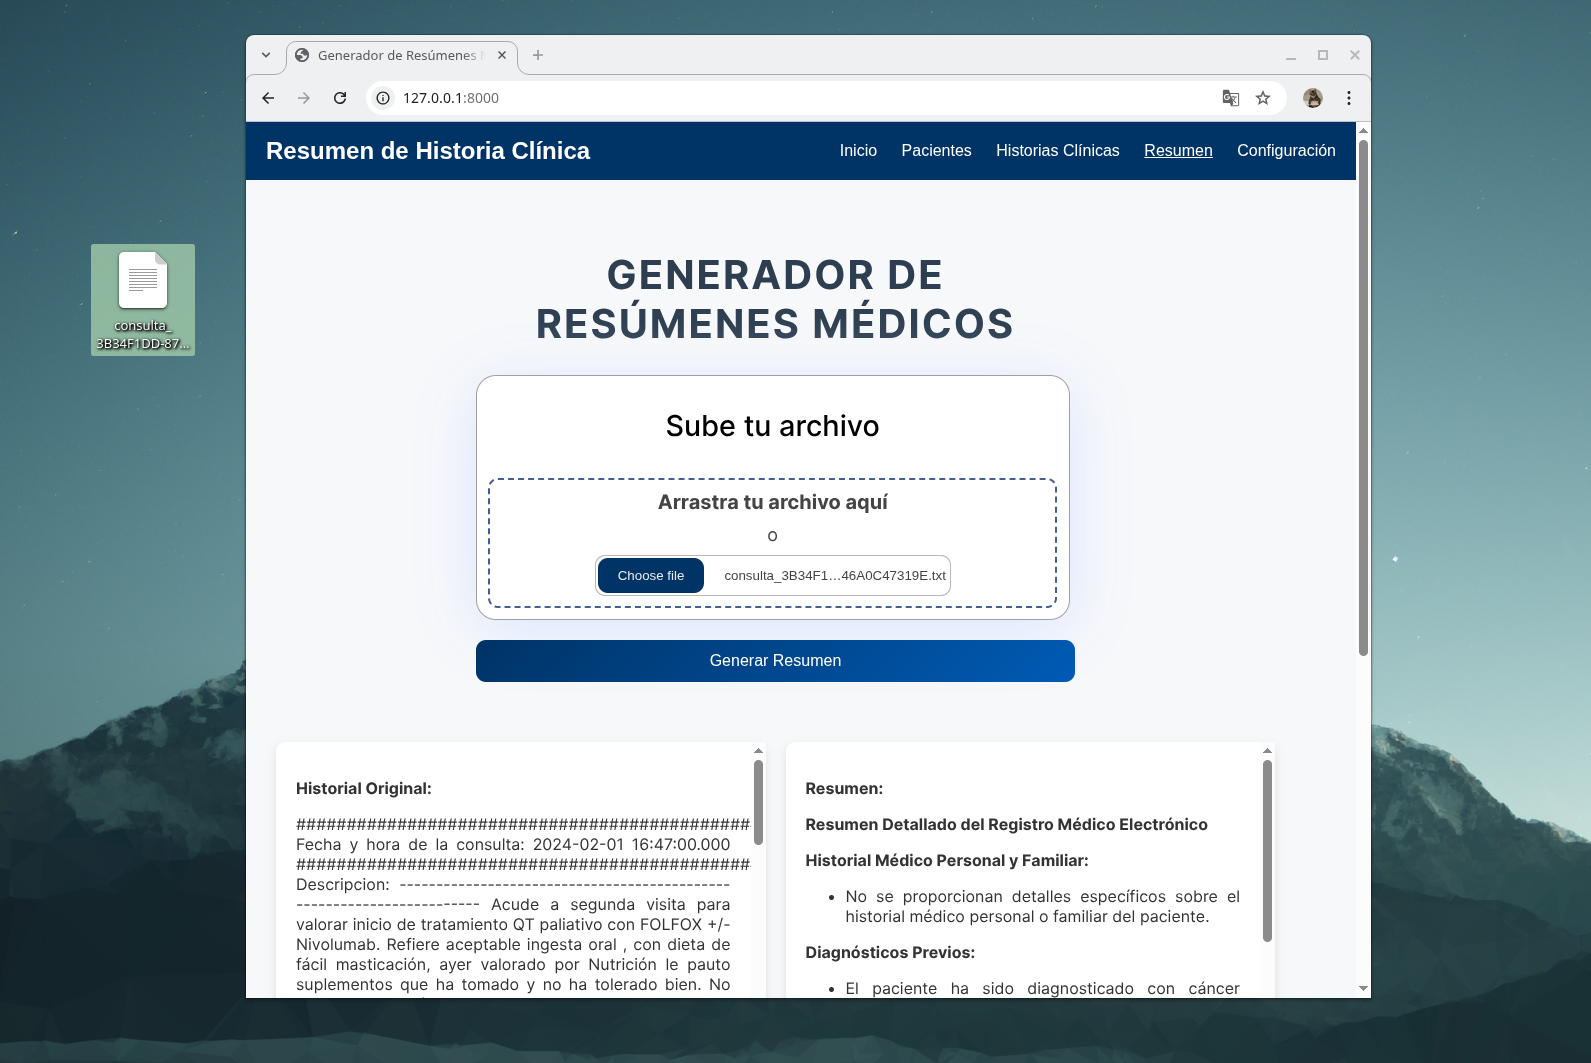
\includegraphics[width=0.8\textwidth]{images/app.png}
	\caption{Interfaz gráfica de la aplicación demostrativa}
	\label{fig:demo_app}
\end{figure}

\end{document}